\documentclass[final,a4paper,10pt,abstracton]{scrreprt}


\usepackage{draftwatermark}\SetWatermarkScale{5} %_DRAFT watermark

%
% General
\usepackage[english]{babel}
\usepackage{hyperref}
\hypersetup{final,plainpages=false,pagebackref,colorlinks=true,linkcolor=blue,urlcolor=red,citecolor=blue,pdfpagemode=UseOutlines,pdfstartview=FitH,pdfborder={0 0 0}}

\providecommand{\indexed}[1]{\index{#1}#1}

\newcommand{\HRule}{\rule{\linewidth}{0.5mm}}
\newcommand{\ie}{i.\,e.\ }
\newcommand{\eg}{e.\,g.\ }

%
% Graphics
\usepackage{pgfpages}
\usepackage{tikz}
\usetikzlibrary{arrows,positioning,shapes,topaths,calc,fit,backgrounds,matrix,shadows,automata}
\usepackage{soul}

%\usetikzlibrary{intersections}
%\usetikzlibrary{calc}
%\usetikzlibrary{positioning}


%
% Snippets 
\usepackage{moreverb}
\usepackage{listings}

% Tables
%-------------
\usepackage{tabularx}



\title{CernVM Release Testing Walkthrough}
% \subtitle{Technical Report}
\author{GNU User}

\providecommand{\cernvmreleasetesting}{{\scshape CernVM Release Testing~}}
\providecommand{\releasetesting}{{\scshape Release Testing~}}
\providecommand{\cern}{{\scshape cern~}}
\providecommand{\cernvm}{{\scshape CernVM~}}
\providecommand{\tapper}{{\scshape Tapper~}}
\providecommand{\amdtapper}{{\scshape AMD Tapper~}}

\providecommand{\todo}[1]{\textcolor{red}{#1}}
\definecolor {light-blue}{rgb}{230,244,255}


\usepackage[nottoc]{tocbibind}

\usepackage{makeidx}
\makeindex

\setcounter{secnumdepth}{4}
\setcounter{tocdepth}{4}

\begin{document}
\selectlanguage{english}
\renewcommand\today{June 2011}

\pagestyle{empty}
\begin{titlepage}
	\begin{addmargin}[-\oddsidemargin]{-\evensidemargin}
  		\newlength{\saveparindent}
		\setlength{\saveparindent}{\parindent}
		\setlength{\parindent}{0cm}

  		\sf
		\center
		\vspace*{-1cm}
		\mbox{
	  		\parbox{4cm}{
				\resizebox{4cm}{!}{\begin{pgfpicture}
\pgfpathmoveto{\pgfqpoint{5.858cm}{9.523cm}}
\pgfpathlineto{\pgfqpoint{16.845cm}{9.523cm}}
\pgfpathlineto{\pgfqpoint{16.845cm}{20.265cm}}
\pgfpathlineto{\pgfqpoint{5.858cm}{20.265cm}}
\pgfpathclose
\pgfusepath{clip}
\begin{pgfscope}
\begin{pgfscope}
\end{pgfscope}
\begin{pgfscope}
\pgfpathmoveto{\pgfqpoint{0cm}{0cm}}
\pgfpathlineto{\pgfqpoint{21cm}{0cm}}
\pgfpathlineto{\pgfqpoint{21cm}{29.7cm}}
\pgfpathlineto{\pgfqpoint{0cm}{29.7cm}}
\pgfpathclose
\pgfusepath{clip}
\definecolor{eps2pgf_color}{rgb}{0.121569,0.337255,0.984314}\pgfsetstrokecolor{eps2pgf_color}\pgfsetfillcolor{eps2pgf_color}
\pgfpathmoveto{\pgfqpoint{8.912cm}{15.808cm}}
\pgfpathcurveto{\pgfqpoint{8.761cm}{15.793cm}}{\pgfqpoint{8.49cm}{15.793cm}}{\pgfqpoint{8.339cm}{15.793cm}}
\pgfpathlineto{\pgfqpoint{8.339cm}{16.471cm}}
\pgfpathlineto{\pgfqpoint{8.851cm}{16.471cm}}
\pgfpathcurveto{\pgfqpoint{8.927cm}{16.471cm}}{\pgfqpoint{9.002cm}{16.456cm}}{\pgfqpoint{9.078cm}{16.456cm}}
\pgfpathcurveto{\pgfqpoint{9.078cm}{16.471cm}}{\pgfqpoint{9.063cm}{16.502cm}}{\pgfqpoint{9.063cm}{16.517cm}}
\pgfpathcurveto{\pgfqpoint{9.063cm}{16.532cm}}{\pgfqpoint{9.078cm}{16.562cm}}{\pgfqpoint{9.078cm}{16.577cm}}
\pgfpathcurveto{\pgfqpoint{9.002cm}{16.577cm}}{\pgfqpoint{8.927cm}{16.562cm}}{\pgfqpoint{8.851cm}{16.562cm}}
\pgfpathlineto{\pgfqpoint{8.339cm}{16.562cm}}
\pgfpathlineto{\pgfqpoint{8.339cm}{17.15cm}}
\pgfpathlineto{\pgfqpoint{8.655cm}{17.15cm}}
\pgfpathlineto{\pgfqpoint{8.912cm}{17.135cm}}
\pgfpathcurveto{\pgfqpoint{8.987cm}{17.135cm}}{\pgfqpoint{9.063cm}{17.12cm}}{\pgfqpoint{9.138cm}{17.12cm}}
\pgfpathcurveto{\pgfqpoint{9.138cm}{17.135cm}}{\pgfqpoint{9.123cm}{17.165cm}}{\pgfqpoint{9.123cm}{17.18cm}}
\pgfpathcurveto{\pgfqpoint{9.123cm}{17.21cm}}{\pgfqpoint{9.138cm}{17.226cm}}{\pgfqpoint{9.138cm}{17.256cm}}
\pgfpathlineto{\pgfqpoint{8.113cm}{17.256cm}}
\pgfpathlineto{\pgfqpoint{8.113cm}{15.687cm}}
\pgfpathlineto{\pgfqpoint{9.153cm}{15.687cm}}
\pgfpathcurveto{\pgfqpoint{9.153cm}{15.702cm}}{\pgfqpoint{9.138cm}{15.732cm}}{\pgfqpoint{9.138cm}{15.748cm}}
\pgfpathcurveto{\pgfqpoint{9.138cm}{15.778cm}}{\pgfqpoint{9.153cm}{15.793cm}}{\pgfqpoint{9.153cm}{15.823cm}}
\pgfpathcurveto{\pgfqpoint{9.078cm}{15.808cm}}{\pgfqpoint{8.987cm}{15.808cm}}{\pgfqpoint{8.912cm}{15.808cm}}
\pgfpathmoveto{\pgfqpoint{11.023cm}{17.256cm}}
\pgfpathlineto{\pgfqpoint{10.933cm}{17.256cm}}
\pgfpathlineto{\pgfqpoint{10.933cm}{15.672cm}}
\pgfpathcurveto{\pgfqpoint{10.948cm}{15.687cm}}{\pgfqpoint{10.978cm}{15.687cm}}{\pgfqpoint{11.008cm}{15.687cm}}
\pgfpathcurveto{\pgfqpoint{11.023cm}{15.687cm}}{\pgfqpoint{11.053cm}{15.687cm}}{\pgfqpoint{11.068cm}{15.672cm}}
\pgfpathlineto{\pgfqpoint{11.068cm}{16.924cm}}
\pgfpathlineto{\pgfqpoint{11.099cm}{16.924cm}}
\pgfpathlineto{\pgfqpoint{12.199cm}{15.823cm}}
\pgfpathcurveto{\pgfqpoint{12.26cm}{15.763cm}}{\pgfqpoint{12.305cm}{15.717cm}}{\pgfqpoint{12.335cm}{15.672cm}}
\pgfpathlineto{\pgfqpoint{12.411cm}{15.672cm}}
\pgfpathlineto{\pgfqpoint{12.411cm}{17.256cm}}
\pgfpathcurveto{\pgfqpoint{12.38cm}{17.256cm}}{\pgfqpoint{12.365cm}{17.241cm}}{\pgfqpoint{12.335cm}{17.241cm}}
\pgfpathcurveto{\pgfqpoint{12.305cm}{17.241cm}}{\pgfqpoint{12.29cm}{17.256cm}}{\pgfqpoint{12.26cm}{17.256cm}}
\pgfpathlineto{\pgfqpoint{12.26cm}{16.064cm}}
\pgfpathlineto{\pgfqpoint{12.245cm}{16.064cm}}
\pgfpathclose
\pgfpathmoveto{\pgfqpoint{7.871cm}{15.928cm}}
\pgfpathcurveto{\pgfqpoint{7.826cm}{15.883cm}}{\pgfqpoint{7.615cm}{15.748cm}}{\pgfqpoint{7.328cm}{15.748cm}}
\pgfpathcurveto{\pgfqpoint{6.936cm}{15.748cm}}{\pgfqpoint{6.65cm}{16.019cm}}{\pgfqpoint{6.65cm}{16.471cm}}
\pgfpathcurveto{\pgfqpoint{6.65cm}{16.848cm}}{\pgfqpoint{6.876cm}{17.195cm}}{\pgfqpoint{7.343cm}{17.195cm}}
\pgfpathcurveto{\pgfqpoint{7.615cm}{17.195cm}}{\pgfqpoint{7.796cm}{17.045cm}}{\pgfqpoint{7.841cm}{16.999cm}}
\pgfpathlineto{\pgfqpoint{7.856cm}{16.999cm}}
\pgfpathcurveto{\pgfqpoint{7.871cm}{17.06cm}}{\pgfqpoint{7.886cm}{17.12cm}}{\pgfqpoint{7.901cm}{17.18cm}}
\pgfpathcurveto{\pgfqpoint{7.735cm}{17.241cm}}{\pgfqpoint{7.539cm}{17.286cm}}{\pgfqpoint{7.358cm}{17.286cm}}
\pgfpathcurveto{\pgfqpoint{6.815cm}{17.286cm}}{\pgfqpoint{6.393cm}{16.984cm}}{\pgfqpoint{6.393cm}{16.471cm}}
\pgfpathcurveto{\pgfqpoint{6.393cm}{15.974cm}}{\pgfqpoint{6.74cm}{15.657cm}}{\pgfqpoint{7.298cm}{15.657cm}}
\pgfpathcurveto{\pgfqpoint{7.494cm}{15.657cm}}{\pgfqpoint{7.705cm}{15.687cm}}{\pgfqpoint{7.856cm}{15.778cm}}
\pgfpathclose
\pgfpathmoveto{\pgfqpoint{9.605cm}{16.532cm}}
\pgfpathlineto{\pgfqpoint{9.605cm}{17.165cm}}
\pgfpathcurveto{\pgfqpoint{9.711cm}{17.165cm}}{\pgfqpoint{9.998cm}{17.18cm}}{\pgfqpoint{10.088cm}{17.165cm}}
\pgfpathcurveto{\pgfqpoint{10.284cm}{17.135cm}}{\pgfqpoint{10.375cm}{17.03cm}}{\pgfqpoint{10.375cm}{16.879cm}}
\pgfpathcurveto{\pgfqpoint{10.375cm}{16.698cm}}{\pgfqpoint{10.239cm}{16.577cm}}{\pgfqpoint{10.043cm}{16.547cm}}
\pgfpathcurveto{\pgfqpoint{9.922cm}{16.517cm}}{\pgfqpoint{9.651cm}{16.532cm}}{\pgfqpoint{9.605cm}{16.532cm}}
\pgfpathmoveto{\pgfqpoint{10.616cm}{15.868cm}}
\pgfpathlineto{\pgfqpoint{10.088cm}{16.471cm}}
\pgfpathcurveto{\pgfqpoint{10.344cm}{16.502cm}}{\pgfqpoint{10.616cm}{16.637cm}}{\pgfqpoint{10.616cm}{16.909cm}}
\pgfpathcurveto{\pgfqpoint{10.616cm}{17.135cm}}{\pgfqpoint{10.435cm}{17.256cm}}{\pgfqpoint{10.043cm}{17.256cm}}
\pgfpathlineto{\pgfqpoint{9.394cm}{17.256cm}}
\pgfpathlineto{\pgfqpoint{9.394cm}{15.672cm}}
\pgfpathcurveto{\pgfqpoint{9.44cm}{15.687cm}}{\pgfqpoint{9.47cm}{15.687cm}}{\pgfqpoint{9.515cm}{15.687cm}}
\pgfpathcurveto{\pgfqpoint{9.545cm}{15.687cm}}{\pgfqpoint{9.59cm}{15.687cm}}{\pgfqpoint{9.621cm}{15.672cm}}
\pgfpathlineto{\pgfqpoint{9.621cm}{16.441cm}}
\pgfpathlineto{\pgfqpoint{9.832cm}{16.441cm}}
\pgfpathlineto{\pgfqpoint{10.028cm}{16.23cm}}
\pgfpathlineto{\pgfqpoint{10.329cm}{15.883cm}}
\pgfpathcurveto{\pgfqpoint{10.39cm}{15.808cm}}{\pgfqpoint{10.435cm}{15.748cm}}{\pgfqpoint{10.495cm}{15.672cm}}
\pgfpathcurveto{\pgfqpoint{10.54cm}{15.687cm}}{\pgfqpoint{10.586cm}{15.687cm}}{\pgfqpoint{10.646cm}{15.687cm}}
\pgfpathcurveto{\pgfqpoint{10.691cm}{15.687cm}}{\pgfqpoint{10.736cm}{15.687cm}}{\pgfqpoint{10.782cm}{15.672cm}}
\pgfpathlineto{\pgfqpoint{10.736cm}{15.732cm}}
\pgfpathclose
\pgfpathmoveto{\pgfqpoint{9.163cm}{12.394cm}}
\pgfpathcurveto{\pgfqpoint{8.998cm}{12.418cm}}{\pgfqpoint{8.836cm}{12.452cm}}{\pgfqpoint{8.677cm}{12.496cm}}
\pgfpathcurveto{\pgfqpoint{9.079cm}{12.099cm}}{\pgfqpoint{9.564cm}{11.791cm}}{\pgfqpoint{10.102cm}{11.601cm}}
\pgfpathlineto{\pgfqpoint{10.285cm}{11.802cm}}
\pgfpathcurveto{\pgfqpoint{9.877cm}{11.933cm}}{\pgfqpoint{9.497cm}{12.134cm}}{\pgfqpoint{9.163cm}{12.394cm}}
\pgfpathmoveto{\pgfqpoint{8.327cm}{17.627cm}}
\pgfpathlineto{\pgfqpoint{8.641cm}{17.624cm}}
\pgfpathcurveto{\pgfqpoint{9.035cm}{18.135cm}}{\pgfqpoint{10.046cm}{18.893cm}}{\pgfqpoint{11.403cm}{18.893cm}}
\pgfpathcurveto{\pgfqpoint{11.698cm}{18.893cm}}{\pgfqpoint{11.985cm}{18.857cm}}{\pgfqpoint{12.259cm}{18.79cm}}
\pgfpathcurveto{\pgfqpoint{12.152cm}{18.903cm}}{\pgfqpoint{12.036cm}{19.008cm}}{\pgfqpoint{11.914cm}{19.106cm}}
\pgfpathcurveto{\pgfqpoint{11.747cm}{19.128cm}}{\pgfqpoint{11.576cm}{19.141cm}}{\pgfqpoint{11.403cm}{19.141cm}}
\pgfpathcurveto{\pgfqpoint{10.19cm}{19.141cm}}{\pgfqpoint{9.068cm}{18.589cm}}{\pgfqpoint{8.327cm}{17.627cm}}
\pgfpathmoveto{\pgfqpoint{11.403cm}{11.624cm}}
\pgfpathcurveto{\pgfqpoint{11.229cm}{11.624cm}}{\pgfqpoint{11.059cm}{11.639cm}}{\pgfqpoint{10.891cm}{11.663cm}}
\pgfpathlineto{\pgfqpoint{10.691cm}{11.444cm}}
\pgfpathcurveto{\pgfqpoint{10.923cm}{11.401cm}}{\pgfqpoint{11.161cm}{11.377cm}}{\pgfqpoint{11.403cm}{11.377cm}}
\pgfpathcurveto{\pgfqpoint{12.506cm}{11.377cm}}{\pgfqpoint{13.503cm}{11.84cm}}{\pgfqpoint{14.21cm}{12.581cm}}
\pgfpathlineto{\pgfqpoint{14.142cm}{12.873cm}}
\pgfpathcurveto{\pgfqpoint{13.475cm}{12.109cm}}{\pgfqpoint{12.495cm}{11.624cm}}{\pgfqpoint{11.403cm}{11.624cm}}
\pgfpathmoveto{\pgfqpoint{14.64cm}{13.119cm}}
\pgfpathcurveto{\pgfqpoint{14.956cm}{13.596cm}}{\pgfqpoint{15.169cm}{14.147cm}}{\pgfqpoint{15.248cm}{14.738cm}}
\pgfpathlineto{\pgfqpoint{15.265cm}{14.736cm}}
\pgfpathlineto{\pgfqpoint{15.889cm}{19.191cm}}
\pgfpathlineto{\pgfqpoint{15.643cm}{19.226cm}}
\pgfpathlineto{\pgfqpoint{15.2cm}{16.058cm}}
\pgfpathcurveto{\pgfqpoint{14.939cm}{17.301cm}}{\pgfqpoint{14.082cm}{18.327cm}}{\pgfqpoint{12.942cm}{18.822cm}}
\pgfpathcurveto{\pgfqpoint{13.044cm}{18.688cm}}{\pgfqpoint{13.138cm}{18.548cm}}{\pgfqpoint{13.223cm}{18.403cm}}
\pgfpathcurveto{\pgfqpoint{14.307cm}{17.773cm}}{\pgfqpoint{15.038cm}{16.6cm}}{\pgfqpoint{15.038cm}{15.259cm}}
\pgfpathcurveto{\pgfqpoint{15.038cm}{14.605cm}}{\pgfqpoint{14.863cm}{13.992cm}}{\pgfqpoint{14.56cm}{13.462cm}}
\pgfpathclose
\pgfpathmoveto{\pgfqpoint{7.769cm}{15.259cm}}
\pgfpathlineto{\pgfqpoint{7.77cm}{15.344cm}}
\pgfpathlineto{\pgfqpoint{7.522cm}{15.35cm}}
\pgfpathlineto{\pgfqpoint{7.521cm}{15.259cm}}
\pgfpathcurveto{\pgfqpoint{7.521cm}{14.938cm}}{\pgfqpoint{7.56cm}{14.619cm}}{\pgfqpoint{7.638cm}{14.31cm}}
\pgfpathcurveto{\pgfqpoint{7.724cm}{13.965cm}}{\pgfqpoint{7.857cm}{13.642cm}}{\pgfqpoint{8.026cm}{13.344cm}}
\pgfpathcurveto{\pgfqpoint{8.161cm}{13.268cm}}{\pgfqpoint{8.303cm}{13.202cm}}{\pgfqpoint{8.448cm}{13.143cm}}
\pgfpathcurveto{\pgfqpoint{8.189cm}{13.506cm}}{\pgfqpoint{7.992cm}{13.918cm}}{\pgfqpoint{7.878cm}{14.371cm}}
\pgfpathcurveto{\pgfqpoint{7.805cm}{14.659cm}}{\pgfqpoint{7.769cm}{14.958cm}}{\pgfqpoint{7.769cm}{15.259cm}}
\pgfpathmoveto{\pgfqpoint{13.376cm}{16.381cm}}
\pgfpathcurveto{\pgfqpoint{13.376cm}{14.377cm}}{\pgfqpoint{11.745cm}{12.747cm}}{\pgfqpoint{9.741cm}{12.747cm}}
\pgfpathcurveto{\pgfqpoint{8.072cm}{12.747cm}}{\pgfqpoint{6.622cm}{13.876cm}}{\pgfqpoint{6.216cm}{15.493cm}}
\pgfpathcurveto{\pgfqpoint{6.144cm}{15.782cm}}{\pgfqpoint{6.107cm}{16.081cm}}{\pgfqpoint{6.107cm}{16.381cm}}
\pgfpathcurveto{\pgfqpoint{6.107cm}{18.385cm}}{\pgfqpoint{7.737cm}{20.016cm}}{\pgfqpoint{9.741cm}{20.016cm}}
\pgfpathcurveto{\pgfqpoint{11.745cm}{20.016cm}}{\pgfqpoint{13.376cm}{18.385cm}}{\pgfqpoint{13.376cm}{16.381cm}}
\pgfpathmoveto{\pgfqpoint{9.741cm}{20.263cm}}
\pgfpathcurveto{\pgfqpoint{7.601cm}{20.263cm}}{\pgfqpoint{5.859cm}{18.522cm}}{\pgfqpoint{5.859cm}{16.381cm}}
\pgfpathcurveto{\pgfqpoint{5.859cm}{16.06cm}}{\pgfqpoint{5.899cm}{15.741cm}}{\pgfqpoint{5.976cm}{15.433cm}}
\pgfpathcurveto{\pgfqpoint{5.984cm}{15.4cm}}{\pgfqpoint{5.995cm}{15.369cm}}{\pgfqpoint{6.004cm}{15.337cm}}
\pgfpathlineto{\pgfqpoint{6.002cm}{15.336cm}}
\pgfpathlineto{\pgfqpoint{6.975cm}{11.854cm}}
\pgfpathlineto{\pgfqpoint{7.214cm}{11.92cm}}
\pgfpathlineto{\pgfqpoint{6.607cm}{14.092cm}}
\pgfpathcurveto{\pgfqpoint{7.321cm}{13.114cm}}{\pgfqpoint{8.47cm}{12.499cm}}{\pgfqpoint{9.741cm}{12.499cm}}
\pgfpathcurveto{\pgfqpoint{10.379cm}{12.499cm}}{\pgfqpoint{10.98cm}{12.654cm}}{\pgfqpoint{11.511cm}{12.928cm}}
\pgfpathlineto{\pgfqpoint{8.408cm}{9.525cm}}
\pgfpathlineto{\pgfqpoint{8.743cm}{9.525cm}}
\pgfpathlineto{\pgfqpoint{12.61cm}{13.765cm}}
\pgfpathlineto{\pgfqpoint{12.608cm}{13.767cm}}
\pgfpathcurveto{\pgfqpoint{13.132cm}{14.341cm}}{\pgfqpoint{13.486cm}{15.073cm}}{\pgfqpoint{13.59cm}{15.882cm}}
\pgfpathlineto{\pgfqpoint{15.075cm}{9.525cm}}
\pgfpathlineto{\pgfqpoint{15.329cm}{9.525cm}}
\pgfpathlineto{\pgfqpoint{13.521cm}{17.264cm}}
\pgfpathlineto{\pgfqpoint{13.521cm}{17.264cm}}
\pgfpathcurveto{\pgfqpoint{13.224cm}{18.532cm}}{\pgfqpoint{12.305cm}{19.564cm}}{\pgfqpoint{11.104cm}{20.016cm}}
\pgfpathlineto{\pgfqpoint{16.843cm}{20.016cm}}
\pgfpathlineto{\pgfqpoint{16.843cm}{20.263cm}}
\pgfusepath{fill}
\end{pgfscope}
\end{pgfscope}
\end{pgfpicture}}
%				
%				%\begin{tikzpicture}[scale=0.5]
%				%	\path[fill=black, join=round] (1,1)--(2,2)--(2,5)--(5,5)--(6,6)--(1,6)--(1,1)--(2,0)--(5,0)--(7,2)--(7,5)--(6,6)--(6,1)--cycle;
%				%	\clip (6,6)--(5,5)--(5,2)--(2,2)--(1,1)--(6,1)--(6,6)--(5,7)--(2,7)--(0,5)--(0,2)--(1,1)--(1,6)--cycle;
%				%	\shade[inner color=green, outer color=black] (3,4) circle(5.5cm);
%				%\end{tikzpicture}
	  		}
	  		\parbox{9cm}{
	    			%\LARGE CERN\\
	    			%\large PH-SFT%\\[0.5cm]
			}
		}
		\vspace*{2.5cm}
 
  		{\large \scshape CernVM Release Testing Walkthrough}\\[0.5cm]
  		\HRule\\[0.4cm]
		\huge CernVM Release Testing\\
		\HRule\\[1.5cm]
		
%        \includegraphics[height=5cm]{marbles}\\[1.5cm]
        
\includegraphics{img/IMG_cernvmlogo}\\[1.5cm] 
		\large GNU User\\[0.4cm]
		%\today
 
		%  \LARGE ---DRAFT---\\[1ex]
		%  \LARGE www.grgen.net\\[6ex]
		%  \LARGE Jakob Blomer \qquad Rubino Gei\ss\\[3ex]
		%  \large \today\\
 
		\large Technical Report\\
		Version: 0.1 (Draft) \today 
		%	\large ISSN 1432-7864	

  		\setlength{\parindent}{\saveparindent}
	\end{addmargin}
\end{titlepage}
\cleardoublepage
\pagenumbering{roman}



\abstract{
The \cernvmreleasetesting\ project is a testing infrastructure for CernVM images, the usecase for the project is to provide an automated
testing environment, which will install and configure CernVM images, run the set of tests and report the results on a web interface.
}

\tableofcontents
\clearpage
\pagenumbering{arabic}
\pagestyle{headings}

\chapter{Overview}
\label{sct:overview}

CernVM currently supports images for VirtualBox, VMware, Xen, KVM and Microsoft Hyper-V hypervisors, each new release of a CernVM image needs to be 
thoroughly tested on each supported platform and hypervisor. The \cernvmreleasetesting\ project is designed to meet this requirement by providing an 
automated testing environment for CernVM images, which will install and configure CernVM images, run the set of tests and report the results on a web
interface.

The intent of this document is to provided a step-by-step guide on setting up an entire \cernvmreleasetesting\ infrastructure, including instructions
on how to set up and configure test clients, the main server running the web interface and database, as well as writing and executing tests. If you are
new to release testing and want a document to guide you through the entire process of setting up a working \cernvmreleasetesting\ infrastructure,
then this guide for you.

All the code needed to setup the entire \releasetesting\ infrastructure for CernVM image testing, is located at the \cernvmreleasetesting\ Google Code project
page\cite{GCreleasetesting} including this document and all other documentation. 

While this document is not intended to be a replacement for the reference manual, the following is a brief description of the \releasetesting\ infrastructure 
including an introduction to the core component, \amdtapper\cite{tapper}. Figure~\ref{fig:architecture} consists of a diagram outlining the
\indexed{\tapper~Architecture}, which consists of test clients and a server, the server is what controls the test clients, gathers 
results, and then displays the results through a web interface.\newline

\begin{figure}[!hbp]
	\begin{center}
		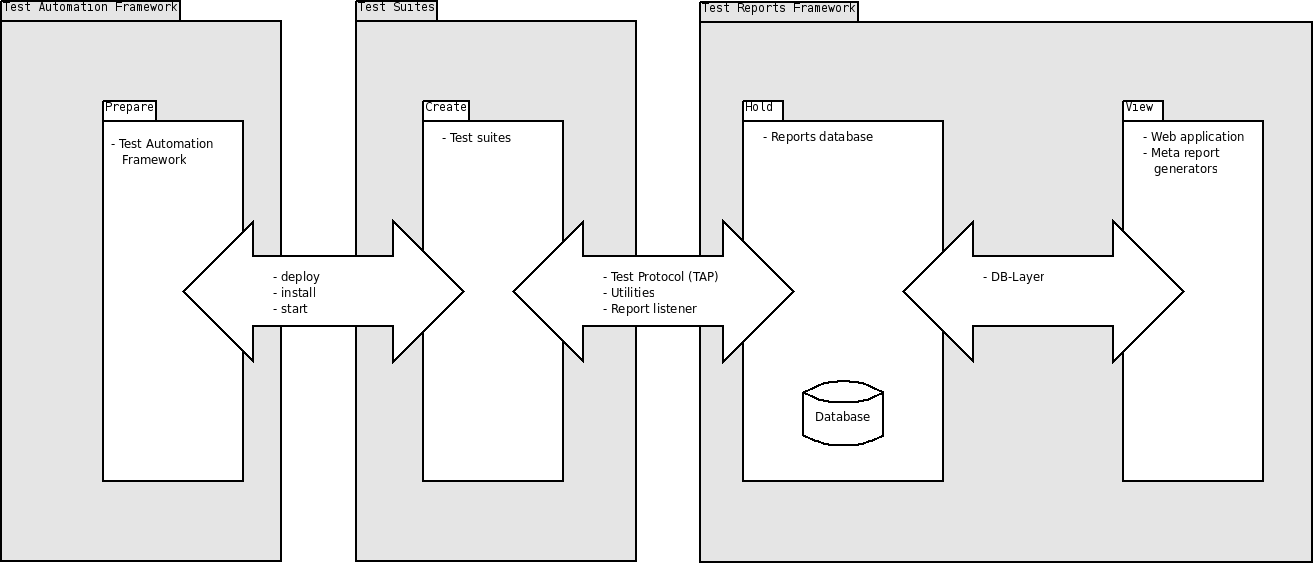
\includegraphics[scale=0.25]{img/tapper_architecture_overview.png}
	\end{center}
	\caption{Overview of the \tapper architecture}
	\label{fig:architecture}
\end{figure}

The components of the \releasetesting~Framework are listed in Table~\ref{tbl:components}. 

\begin{table}
  \begin{center}

    \begin{tabularx}{\linewidth}{l|X}
      {\bf\centering \releasetesting component name} & {\bf\centering Description} \\\hline
%        \texttt{Agent} & Communicates with service insances and requests a job to execute. Upon receiving the job downloads the input 
%                         files, executes the job, uploads job output files and reports that the job execution is finished. \\
%        \texttt{Generic Job and Storage Manager} & Distributes jobs from the internal queue to Agents for execution, provides space for storing 
%                                                   the job output   \\
%        \texttt{AliEn Job Manager} & Retrieves jobs from the central task queue of \indexed{AliEn} Grid \cite{alien} and sends them to 
%                                     Agents for execution \\
%        \texttt{AliEn Storage Manager} & Uploads the output of AliEn jobs executed by Agents and finalizes the job status in AliEn Grid.  \\
%        \texttt{PanDA Storage Manager} & Uploads the output of \indexed{PanDA} \cite{panda} jobs executed by Agents and finalizes the job status in PanDA Grid  \\
    \end{tabularx}  
  \end{center}

  \caption{List of \releasetesting and \amdtapper components}

  \label{tbl:components}
\end{table}

\chapter{\cernvmreleasetesting Test Client Platform Setup}
\label{sec:testclientsetup}

\section{Introduction}
The intent of this document is to provided a step-by-step guide on setting up an entire \cernvmreleasetesting\ infrastructure, including 
instructions on how to set up and configure test clients, the main server running the web interface and database, as well as writing and 
executing tests. If you are new to release testing and want a document to guide you through the entire process of setting up a working
 \cernvmreleasetesting\ infrastructure, then this guide for you.

This section provides complete step by step instructions on how to setup and configure the test clients which are part of a basic working
\releasetesting environment by outlining the procedure for setting up test clients on numerous platforms, hence why this is called a 
\emph{walkthrough} document. This guide is intended for users familiar enough with computers and desktop environments to enter basic commands
in a terminal and install various operating systems. 

As this guide is directed towards users who are new to \cernvmreleasetesting and \tapper and
are interested in quickly getting a \cernvm testing infrastructure quickly set up, many assumptions regarding the requirements necessary are 
made.As is the case, these instructions are provided for a generalized audience based on our own experience and the requirements that we feel 
most users will have, \emph{so feel free to deviate from the instructions}.
\chapter{\cernvmreleasetesting Server Platform Setup}
\label{sct:serversetup}

\section{Introduction}
This section provides complete step by step instructions on how to setup and configure the \tapper server which are part of a basic working
\releasetesting environment by outlining the procedure for setting up the server, hence why this is called a \emph{walkthrough} document. 
This guide is intended for users familiar enough with computers and desktop environments to enter basic commands in a terminal and install 
various operating systems. 

\section{Red Hat Based Server Setup}
\subsection{Installing the system}
\subsection{Configuring the system}
\subsection{Installing the Tapper Server}
\subsection{Setting up Tapper Web Interface and Database}

\section{Debian Based Server Setup}
\subsection{Installing the system}
\subsection{Configuring the system}
\subsection{Installing the Tapper Server}
\subsection{Setting up Tapper Web Interface and Database}


\pagestyle{plain}
\bibliographystyle{plain}
\bibliography{walkthroughRefs,rfc}

\printindex

\end{document}
